\chapter{Quality Assessment}
\label{chap:qualityassessment}

In this chapter, we begin by examining related work in the field of \gls{iqa}.
We then review the specific metrics used in our thesis to evaluate the performance of \gls{iqa} algorithms.

\section{Conventional Quality Assessment}

\Gls{iqa} is a research field dedicated to quantifying the quality of distorted images \cite{iqa_survey_2020}.
The term "quality" always refers to the quality of an image as perceived by the human visual system.
However, there is an exception when images are used for machine learning or other tasks that do not involve human perception.
In this cases, image quality may be defined by the performance of the machine learning algorithm.
This aspect becomes crucial when determining the appropriate compression techniques for datasets used in machine learning or identifying the types of distortions that have the most significant impact on \gls{ocr} algorithms.
Consider, for instance, an application where an \gls{ocr} algorithm is utilized to recognize text in a presentation, and the recognized text is then read aloud by a text-to-speech system for a blind person.
In this scenario, the image quality is defined by the performance of the \gls{ocr} algorithm rather than human perception.

Generally, we can divide \gls{iqa} algorithms into three categories: \gls{fr}, \gls{rr} and \gls{nr}.
The goal of \gls{fr} algorithms is to predict the quality of a distorted image by comparing it to the reference image.
\Gls{rr} algorithms predict the quality of the distorted image by comparing a reduced number of features of the distorted image to the reference image.
\Gls{nr} algorithms only use the distorted image to predict its quality.
In this thesis, we focus on \gls{fr} algorithms, as we have access to the original images.
Another distinction can be made between the type of images that are used for the evaluation.
We can differentiate between natural images and \gls{sci}.
Natural images can be pictures of landscapes, people or objects.

For natural images, one common metric is the \gls{psnr} \cite{PSNRvsSSIM_2010}.
It describes the ratio of the maximum possible power of a signal and the power of corrupting noise that affects it.
When it is applied to an image, the \gls{psnr} is defined as follows.

\begin{equation}
    \text{PSNR} = 10 \cdot \log_{10} \left( \frac{R^2}{\text{MSE}} \right),
    \label{eq:psnr}
\end{equation}

with \(R\) being the maximum possible pixel value of the image and MSE being the \gls{mse} between the original and the reconstructed image.

Another common metric is the \gls{ssim} \cite{SSIM_2004}, which combines the luminance, the contrast and the structural differences between two images into one metric.
Compared to the \gls{psnr}, the \gls{ssim} is more closely correlated with human perception of image quality \cite{frmetric_comp_2012}.

--- maybe FSIM


\section{Screen Content Specific Quality Assessment}

A neighboring field is document image quality assessment, which assesses the quality of scanned documents and is thus mainly concerned with text \cite{3_subj_weight_2015}.
\Glspl{sci} are images that contain text, graphics and user interface elements.
They often contain a combination of document and natural image content.
Therefore, because they differ statistically from natural and document images, different metrics are required to evaluate their quality.
To address this issue, some research has been conducted.

Researchers used a convolutional neural network to assess the quality of documents \cite{ocr_cnn_docu_2014}.
The documents were segmented into text and non-text regions.
Then \gls{ocr} and the proposed \gls{cnn} were used to predict scores, which were analyzed for correlation.
The \gls{cnn} achieved state of the art performance in assessing the quality of the documents.
However, the authors noted that one assumption was, that the \gls{ocr} performance is directly correlated with the quality of the degraded document.
% Due to the similarity of text regions in documents and screen content, we might be able to verify or disprove this assumption in this thesis.

In \cite{text_pict_weight_2017}, the authors propose an objective metric that considers the text and pictorial content of an image separately.
Afterwards, the two scores are weighted and combined.

Yang et al. \cite{3_subj_weight_2015} use a subjective score, that considers text, pictorial and the entire image separately.
The correlation between the three scores is then analyzed, weighted and used to combine them into a single score.

% --- most papers use ocr as a comparison, almost like ground truth, or predict when ocr is good


\section{Evaluation Procedure of Quality Assessment Algorithms}
\label{sec:evalprocedure}

To evaluate the suitability of an objective \gls{iqa} method, in our case the $\text{CER}_{\text{c}}$, see \autoref{subsec:cer}, and its correlation to the human subjective score, in this thesis the \gls{mos}, see \autoref{chap:dataset}, there are three aspects to consider \cite{nonlin_fit_original_2003}\cite{iqa_survey_2020}.
Prediction consistency, prediction monotonicity, and prediction accuracy.

\subsection{Nonlinear Transformation}
\label{subsec:nonlinear}

Before calculating metrics to measure these aspects, the \gls{vqeg} recommends removing nonlinearities from the \gls{mos} \cite{nonlin_fit_original_2003}.
To do this, we fit a model to the $\text{CER}_{\text{c}}$ and the \gls{mos} values.
This model is described in \cite{nonlin_fit_model_init_2000}\cite{nonlin_fit_appl_2017}.
Given the $i$-th image in our dataset, its \gls{mos} value is denoted as $\text{MOS}_{i}$, its $\text{CER}_{\text{c}}$ value as $\text{CER}_{\text{c},i}$ and its predicted \gls{mos} value as $\text{MOS}_{\text{p},i}$.
The corresponding vectors are defined as
\begin{equation}
    \mathbf{CER}_{\text{c}} =
    \begin{pmatrix}
        \text{CER}_{\text{c},1} \\
        \text{CER}_{\text{c},2} \\
        \vdots \\
        \text{CER}_{\text{c},N}
    \end{pmatrix},\text{ }
    \mathbf{MOS} =
    \begin{pmatrix}
        \text{MOS}_{1} \\
        \text{MOS}_{2} \\
        \vdots \\
        \text{MOS}_{N}
    \end{pmatrix} \text{ and }
    \mathbf{MOS}_{\text{p}} =
    \begin{pmatrix}
        \text{MOS}_{\text{p},1} \\
        \text{MOS}_{\text{p},2} \\
        \vdots \\
        \text{MOS}_{\text{p},N}
    \end{pmatrix}.
\end{equation}

Then the model can be defined as

\begin{equation}
    \mathbf{MOS}_{\text{p}} = \frac{\beta_{1}-\beta_{2}}{1 + \text{e}^{-\left(\frac{\mathbf{CER}_{\text{c}}-\beta_{3}}{|\beta_{4}|}\right)}} + \beta_{2},
    \label{eq:nonlinear}
\end{equation}

% \begin{equation}
%     s_{i,p} = a * (\frac{1}{2} - \frac{1}{1 + \exp{b * (x - c)}}) + d * x + e
%     \label{eq:nonlinear}
% \end{equation}

with $\beta_{1}$, $\beta_{2}$, $\beta_{3}$, and $\beta_{4}$ denoting the parameters of the model.

Although the model in \cite{nonlin_fit_original_2003} is more recent, we could not find initial parameters for it and decided to work with the older model.
Additionally, there are other, more recent, publications \cite{ni_esim_2017, nonlin_fit_appl_2017, nonlin_fit_appl_2018, nonlin_fit_appl_2014, nonlin_fit_appl_2011, nonlin_fit_appl_2015, doc_quality_survey_2023, iqa_database_2023, nonlin_fit_appl_2016} that use the model proposed in \cite{nonlin_fit_new_model_2006}.
In \cite{nonlin_fit_init_proof_2017}, a solution to estimating the initial parameters is proposed, which is out of scope for this thesis.

% --- random, empirical selection can lead to local optimal solutions, which is inconsistent, and maybe a bad comparison basis

The parameters are initialized as
 
\begin{equation}
    \begin{aligned}
        \beta_{1} &= \max{\mathbf{CER}_{\text{c}}} \\
        \beta_{2} &= \min{\mathbf{CER}_{\text{c}}} \\
        \beta_{3} &= \overline{\text{MOS}} \\
        \beta_{4} &= 1.
    \end{aligned}
    \label{eq:nonlinear_init}
\end{equation}
The parameters are adjusted with the least squared method until the model fits the data of all the images.
The model and the $\text{CER}_{\text{c}}$ values are then used to calculate the predicted \gls{mos} values $\text{MOS}_{\text{p}}$.

\begin{figure}[h]
    \centering
    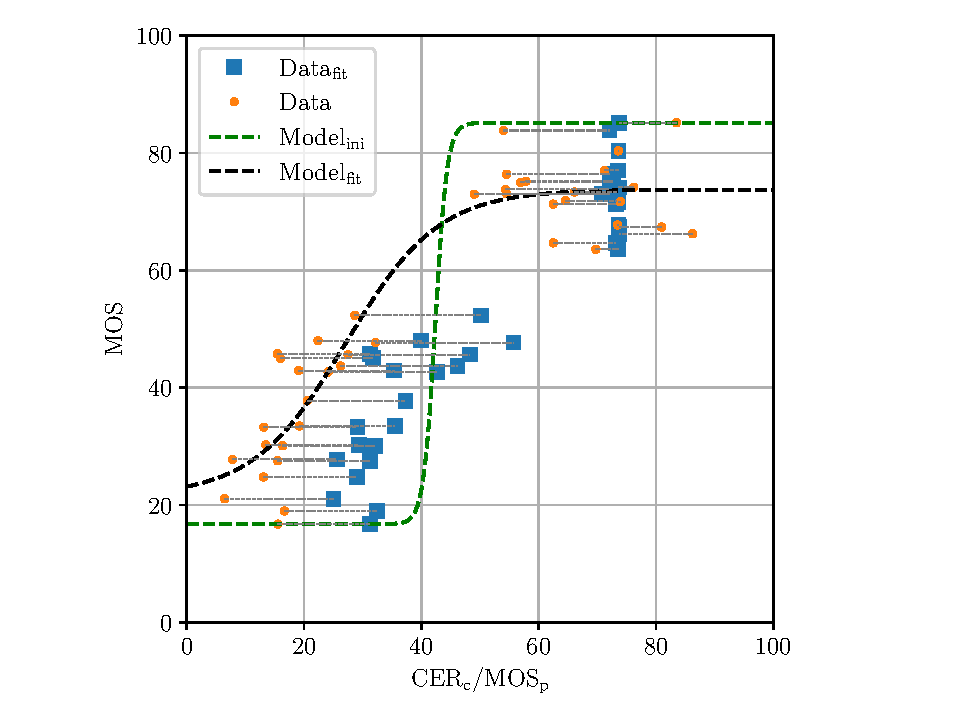
\includegraphics[width=\textwidth]{../exp/fit_example.pdf}
    \caption{Example of the nonlinear fitting. Data before fitting ($\text{CER}_{c}$ vs. \gls{mos}) and after fitting ($\text{MOS}_{p}$ vs \gls{mos}). Model with initial parameters and fitted parameters.}
    \label{fig:nonlinear_fit}
\end{figure}

In Figure \ref{fig:nonlinear_fit} an example of the nonlinear fitting is depicted.
The initial data consists of some randomly generated dummy \gls{mos} and $\text{CER}_{\text{c}}$ values.
We can see, that the model with the initial parameters does not fit the data.
The parameters are then adjusted by the least squares method \cite{least_squares_1978} to fit the model to the data.
Finally, we can see that the fitted curve clearly fits the data better than the curve with the initial parameters.
Now the $\text{MOS}_{\text{p}}$ values can be calculated by using the fitted model and the $\text{CER}_{\text{c}}$ values.
With the $\text{MOS}_{\text{p}}$ the following three metrics \cite{iqa_survey_2021} can be calculated.

\subsection{Pearson Correlation}
\label{subsec:pearson}

The \gls{plcc} \cite{pears_spear_2016} describes the linear correlation between two variables, normalized to the range $[-1, 1]$.
It is defined as

\begin{equation}
    \text{PLCC} = \frac{\sum_{i=1}^{N}{(\text{MOS}_{i}-\overline{\text{MOS}})(\text{MOS}_{\text{p},i}-\overline{\text{MOS}}_{\text{p}})}}{\sqrt{\sum_{i=1}^{N}{(\text{MOS}_{i}-\overline{\text{MOS}})^2}\sum_{i=1}^{N}{(\text{MOS}_{\text{p},i}-\overline{\text{MOS}}_{\text{p}})^2}}},
    \label{eq:pearson}
\end{equation}

with $\overline{\text{MOS}}$ and $\overline{\text{MOS}}_{\text{p}}$ representing the mean values of the $\mathbf{MOS}$ and $\mathbf{MOS}_{\text{p}}$ vectors respectively and $N$ the total number of images in the dataset.
$N$ is the total number of images in the images used in the experiment.
If the \gls{plcc} is close to 1, the two vectors have a positive linear relationship, which means that if $\text{MOS}_{i}$ increases, $\text{MOS}_{\text{p},i}$ increases as well.
If the \gls{plcc} is close to -1, the two vectors have a negative linear relationship, which means that if $\text{MOS}_{i}$ increases, $\text{MOS}_{\text{p},i}$ decreases.
If the \gls{plcc} is close to 0, the two vectors have no correlation at all.
% We are using the sample form of the correlations, because we want to make a statement about a much larger population of images, not just our dataset.

\subsection{Spearman Ranked Correlation}
\label{subsec:spearman}

The \gls{srcc} \cite{pears_spear_2016} describes the monotonic correlation between two variables, normalized to the range $[-1, 1]$.
Compared to the \gls{plcc}, it mainly takes the rank, or order, of the values into account, not the exact values.
The scores $\text{CER}_{\text{c},i}$ and $\text{MOS}_{i}$ are transformed into their ranks $\text{CER}_{\text{c,r},i}$ and $\text{MOS}_{\text{r},i}$ respectively, with values in the range $[1, N]$.
If for example, the first two values are tied, their rank is set to the mean, in this case $(1+2)/2 = 1.5$.
With these values, the \gls{srcc} is defined as

\begin{equation}
    \text{SRCC} = \frac{\sum_{i=1}^{N}{(\text{MOS}_{\text{r},i}-\overline{\text{MOS}}_{\text{r}})(\text{CER}_{\text{c,r},i}-\overline{\text{CER}}_{\text{c,r}})}}{\sqrt{\sum_{i=1}^{N}{(\text{MOS}_{\text{r},i}-\overline{\text{MOS}}_{\text{r}})^2}\sum_{i=1}^{N}{(\text{CER}_{\text{c,r},i}-\overline{\text{CER}}_{\text{c,r}})^2}}},
    \label{eq:spearman}
\end{equation}

with $\overline{\text{MOS}}_{\text{r}}$ and $\overline{\text{CER}}_{\text{c,r}}$ representing the mean values of the $\mathbf{MOS}_{\text{r}}$ and $\mathbf{CER}_{\text{c,r}}$ vectors respectively.
If the \gls{srcc} is close to 1, the two vectors have a positive monotonic relationship, which means that the rank of $\text{CER}_{\text{c},i}$ increases, while the rank of $\text{MOS}_{i}$ increases.
If the \gls{srcc} is close to -1, the two vectors have a negative monotonic relationship, which means that the rank of $\text{CER}_{\text{c},i}$ increases, while the rank of $\text{MOS}_{i}$ decreases.
If the \gls{srcc} is close to 0, the ranks of the two vectors have no correlation at all.
These characteristics will help us to determine if the $\text{CER}_{\text{c}}$ is a good predictor for the \gls{mos}, by checking how similar the ranks of the two metrics are.


\subsection{Root Mean Squared Error}
\label{subsec:rmse}

The \gls{rmse} is a metric that measures the average magnitude of the error between the predicted values and the actual values.
In our case it is defined as

\begin{equation}
    \text{RMSE} = \sqrt{\frac{1}{N}\sum_{i=1}^{N}{(\text{MOS}_{\text{p},i} - \text{MOS}_{i})^2}}.
    \label{eq:rmse}
\end{equation}

From these metrics, \gls{plcc} measures the prediction linearity and consistency, \gls{srcc} measures the prediction monotonicity and the \gls{rmse} measures the prediction accuracy.
With these, we can now determine if the $\text{CER}_{\text{c}}$ is a good predictor for the \gls{mos}.
It is a better predictor the larger \gls{plcc} and \gls{srcc} values are, and the smaller the \gls{rmse} is.


\section{Bjøntegaard Delta Rate}
\label{subsec:bdrate}

The \gls{bdrate} \cite{bdrate_original_2001}\cite{bdrate_beyond_2022} is defined as the average difference between two rate-distortion curves of two codecs to compare.
The first curve is the reference curve and the second the test curve.
Those curves are defined by a set of points $(R_{\text{k,i}}, M_{\text{k,i}})$, where $R_{\text{k,i}}$ is the bitrate and $M_{\text{k,i}}$ is the metric of the image compressed by the codec $k$, with $k /in \{A,B\}$, with \gls{qp} $i$, with $i \in \{35,40,45,50\}$.
The $R_{\text{k,i}}$ values are first converted to the logarithmic scale to not bias the results towards the higher bitrates with

\begin{equation}
    r_{\text{k,i}} = \log_{10}\left(R_{\text{k,i}}\right).
    \label{eq:log_scale}
\end{equation}

Those values in combination with the corresponding $M_{\text{k,i}}$ values are then used as anchor points for an interpolation with a third order polynomial.
The resulting functions are denoted by $\hat{r}_{\text{k}}$, respectively.
The interpolation results in two curves, one for each codec, that pass through all anchor points.

Finally, the \gls{bdrate} can be denoted as $\Delta R$ and is calculated by the integral of the difference between the two curves as

\begin{equation}
    \Delta R = 10^{\frac{1}{M_{\text{low}}-M_{\text{high}}} \int_{M_{\text{low}}}^{M_{\text{high}}} \hat{r}_{\text{B}}(M) - \hat{r}_{\text{A}}(M) \text{d}M} - 1.
    \label{eq:bdrate}
\end{equation}

The lower and upper bound of the integral are given by

\begin{equation}
    \begin{aligned}
        M_{\text{low}} = \max\left(M_{\text{A},50}, M_{\text{B},50}\right) \\
        M_{\text{high}} = \min\left(M_{\text{A},35}, M_{\text{B},35}\right).
    \end{aligned}
    \label{eq:bounds}
\end{equation}

The bounds are the maximum of the lowest quality points and the minimum of the highest quality points and can be seen in \autoref{fig:bdrate_example}.


$\Delta R$ describes the average difference between the two curves in percent.
This enables us to compare the rate-distortion curves of two codecs.
In our case, we can calculate the $\text{CER}_{\text{c}}$ for each codec, once in relation to the \gls{gt} and once in relation to the \gls{ocr} prediction on the reference image.
These two values can then be compared to evaluate, if using the \gls{ocr} algorithms as a reference is a good estimation of the difference between codecs.
If the difference between the two values is small, then the estimation is good and we might be able to use the \gls{ocr} algorithms as a reference for future codec comparisons.
We go into more detail about the codecs we use for our comparisons in \autoref{sec:dataset_codec}.

In this chapter we have defined the metrics to evaluate the predicted $\text{CER}_{\text{c}}$ values.
However, to calculate the $\text{CER}_{\text{c}}$ values, we need \gls{ocr} algorithms to extract text from the images.
Thus, in the following chapter we introduce the \gls{ocr} algorithms that we use in our experiments.
